\documentclass[tikz,border=2pt]{standalone}
\usepackage{amsmath,amssymb}
\usepackage{tikz}
\usetikzlibrary{arrows.meta}

\begin{document}
% Basic feasible solutions = basic solutions with all variables >= 0 = the corners of the
% feasible polygon; basic solutions with a negative variable are intersections outside it.
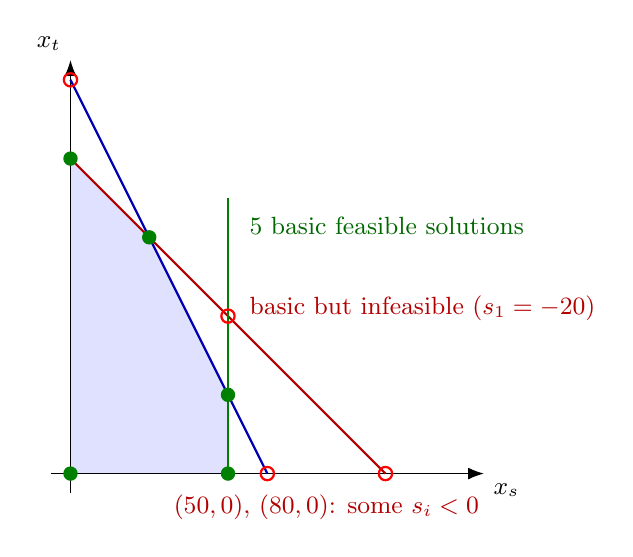
\begin{tikzpicture}[x=0.05cm, y=0.05cm, every node/.style={font=\small}, >={Latex[length=2mm]}]
	\fill[blue!12] (0,0) -- (40,0) -- (40,20) -- (20,60) -- (0,80) -- cycle;
	\draw[->] (-5,0) -- (105,0) node[below right] {$x_s$};
	\draw[->] (0,-5) -- (0,105) node[above left] {$x_t$};
	\draw[blue!70!black, thick] (50,0) -- (0,100);
	\draw[red!70!black, thick] (80,0) -- (0,80);
	\draw[green!50!black, thick] (40,0) -- (40,70);
	\foreach \p in {(0,0),(40,0),(40,20),(20,60),(0,80)} {\fill[green!50!black] \p circle (2.6pt);}
	\node[green!40!black, font=\small, anchor=west] at (43,63) {$5$ basic feasible solutions};
	\foreach \p in {(50,0),(80,0),(0,100),(40,40)} {\draw[red, thick] \p circle (2.4pt);}
	\node[red!70!black, font=\small, anchor=west] at (43,42) {basic but infeasible ($s_1=-20$)};
	\node[red!70!black, font=\small, anchor=north] at (65,-3) {$(50,0)$, $(80,0)$: some $s_i<0$};
	\end{tikzpicture}
\end{document}
